%
% Template Laporan Skripsi/Thesis 
%
% @author  Andreas Febrian, Lia Sadita 
% @version 1.03
%
% Dokumen ini dibuat berdasarkan standar IEEE dalam membuat class untuk 
% LaTeX dan konfigurasi LaTeX yang digunakan Fahrurrozi Rahman ketika 
% membuat laporan skripsi. Konfigurasi yang lama telah disesuaikan dengan 
% aturan penulisan thesis yang dikeluarkan UI pada tahun 2008.
%

%
% Tipe dokumen adalah report dengan satu kolom. 
%
\documentclass[12pt, a4paper, onecolumn, oneside, final]{report}

% Load konfigurasi LaTeX untuk tipe laporan thesis
\usepackage{uithesis}


% Load konfigurasi khusus untuk laporan yang sedang dibuat
%-----------------------------------------------------------------------------%
% Informasi Mengenai Dokumen
%-----------------------------------------------------------------------------%
% 
% Judul laporan. 
\var{\judul}{Implementasi \SCM Sistem Informasi Penjualan Pada Toko Chaca Komputer Jambi}
% 
% Tulis kembali judul laporan, kali ini akan diubah menjadi huruf kapital
\Var{\Judul}{Implementasi \f{Supply Chain Management} Sistem Informasi Penjualan Pada Toko Chaca Komputer Jambi}
% 
% Tulis kembali judul laporan namun dengan bahasa Ingris
\var{\judulInggris}{Unknown Title for Final Report/Thesis/Disertation}

% 
% Tipe laporan, dapat berisi Skripsi, Tugas Akhir, Thesis, atau Disertasi
\var{\type}{Thesis}
% 
% Tulis kembali tipe laporan, kali ini akan diubah menjadi huruf kapital
\Var{\Type}{Thesis}
% 
% Tulis nama penulis 
\var{\penulis}{Ade Indra Saputra}
% 
% Tulis kembali nama penulis, kali ini akan diubah menjadi huruf kapital
\Var{\Penulis}{Ade Indra Saputra}
% 
% Tulis NPM penulis
\var{\npm}{75118017}
% 
% Tuliskan Fakultas dimana penulis berada
\Var{\Fakultas}{Pascasarjana}
\var{\fakultas}{Pascasarjana}
% 
% Tuliskan Program Studi yang diambil penulis
\Var{\Program}{Magister Sistem Informasi}
\var{\program}{Magister Sistem Informasi}
% 
% Tuliskan tahun publikasi laporan
\Var{\bulanTahun}{Januari 2020}
% 
% Tuliskan gelar yang akan diperoleh dengan menyerahkan laporan ini
\var{\gelar}{Magister Komputer}
% 
% Tuliskan tanggal pengesahan laporan, waktu dimana laporan diserahkan ke 
% penguji/sekretariat
\var{\tanggalPengesahan}{XX Januari 2010} 
% 
% Tuliskan tanggal keputusan sidang dikeluarkan dan penulis dinyatakan 
% lulus/tidak lulus
\var{\tanggalLulus}{XX Januari 2010}
% 
% Tuliskan pembimbing 
\var{\pembimbing}{Prof. XXXX}
% 
% Alias untuk memudahkan alur penulisan paa saat menulis laporan
\var{\saya}{Penulis}

%-----------------------------------------------------------------------------%
% Judul Setiap Bab
%-----------------------------------------------------------------------------%
% 
% Berikut ada judul-judul setiap bab. 
% Silahkan diubah sesuai dengan kebutuhan. 
% 
\Var{\kataPengantar}{Kata Pengantar}
\Var{\babSatu}{Pendahuluan}
\Var{\babDua}{Landasan Teori}
\Var{\babTiga}{Metodelogi Penelitian}
\Var{\babEmpat}{Analisis dan Pembahasan}
\Var{\babLima}{Penutup}
%\Var{\babEnam}{Hasil Penelitian}
%\Var{\kesimpulan}{Kesimpulan dan Saran}

% Daftar pemenggalan suku kata dan istilah dalam LaTeX
\include{hype.indonesia}
% Daftar istilah yang mungkin perlu ditandai 
%
% @author  Andreas Febrian
% @version 1.00
% 
% Mendaftar seluruh istilah yang mungkin akan perlu dijadikan 
% italic atau bold pada setiap kemunculannya dalam dokumen. 
% 

\var{\license}{\f{Creative Common License 1.0 Generic}}
\var{\bslash}{$\setminus$}
\var{\SCM}{\f{Supply Chain Management }}
\var{\scm}{\f{SCM }}

% Awal bagian penulisan laporan
\begin{document}
%
% Sampul Laporan
%
% Sampul Laporan

%
% @author  unknown
% @version 1.01
% @edit by Andreas Febrian
%

\begin{titlepage}
    \begin{center}    
        \begin{figure}
            \begin{center}
                
\includegraphics[width=2.5cm]{pics/unikom-black.png}
            \end{center}
        \end{figure}    
        \vspace*{0cm}
        \bo{
        	UNIVERSITAS KOMPUTER INDONESIA\\
        }
        
        \vspace*{1.0cm}
        % judul thesis harus dalam 14pt Times New Roman
        \bo{\Judul} \\[1.0cm]

        \vspace*{2.5 cm}    
        % harus dalam 14pt Times New Roman
        \bo{\Type}

        \vspace*{3 cm}       
        % penulis dan npm
        \bo{\Penulis} \\
        \bo{\npm} \\

        \vspace*{5.0cm}

        % informasi mengenai fakultas dan program studi
        \bo{
        	FAKULTAS \Fakultas\\
        	PROGRAM STUDI \Program \\
        	BANDUNG \\
        	\bulanTahun
        }
    \end{center}
\end{titlepage}


%
% Gunakan penomeran romawi
\pagenumbering{roman}

%
% load halaman judul dalam
\addChapter{HALAMAN JUDUL}
%
% Halaman Judul Laporan 
%
% @author  unknown
% @version 1.01
% @edit by Andreas Febrian
%

\begin{titlepage}
    \begin{center}\begin{figure}
            \begin{center}
                
\includegraphics[width=2.5cm]{pics/unikom-black.png}
            \end{center}
        \end{figure}    
        \vspace*{0cm}
        \bo{
        	UNIVERSITAS KOMPUTER INDONESIA\\
        }
        
        \vspace*{1.0cm}
        % judul thesis harus dalam 14pt Times New Roman
        \bo{\Judul} \\[1.0cm]

        \vspace*{2.5 cm}    
        % harus dalam 14pt Times New Roman
        \bo{\Type} \\
        % keterangan prasyarat
        \bo{Diajukan sebagai salah satu syarat untuk memperoleh gelar \\
        \gelar}\\

        \vspace*{3 cm}       
        % penulis dan npm
        \bo{\Penulis} \\
        \bo{\npm} \\

        \vspace*{5.0cm}

        % informasi mengenai fakultas dan program studi
        \bo{
        	FAKULTAS \Fakultas\\
        	PROGRAM STUDI \Program \\
        	BANDUNG \\
        	\bulanTahun
        }
    \end{center}
\end{titlepage}

%
% setelah bagian ini, halaman dihitung sebagai halaman ke 2
\setcounter{page}{2}

%
% load halaman pengesahan
\addChapter{LEMBAR PERSETUJUAN}
\include{pengesahan}
%
% load halaman orisinalitas 
\addChapter{LEMBAR PERNYATAAN ORISINALITAS}
\include{orisinal}
%
%
\addChapter{LEMBAR PENGESAHAN}
\include{pengesahan_sidang}
%
%
\addChapter{\kataPengantar}
%-----------------------------------------------------------------------------%
\chapter*{\kataPengantar}
%-----------------------------------------------------------------------------%
Template ini disediakan untuk orang-orang yang berencana menggunakan 
\latex~untuk membuat dokumen tugas akhirnya. 
Mengapa \latex? 
Ada banyak hal mengapa menggunakan \latex, diantaranya:

\begin{enumerate}
	\item \latex~membuat kita jadi lebih fokus terhadap isi dokumen, bukan 
		tampilan atau halaman. 
	\item \latex~memudahkan dalam penulisan persamaan matematis. 
	\item Adanya automatis dalam penomoran caption, bab, subbab, subsubbab, 
		referensi, dan rumus. 
	\item Adanya automatisasi dalam pembuatan daftar isi, daftar gambar, dan
		daftar tabel. 
	\item Adanya kemudahan dalam memberikan referensi dalam tulisan dengan 
		menggunakan label. Cara ini dapat meminimalkan kesalahan pemberian 
		referensi. 
\end{enumerate}

Template ini bebas digunakan dan 
didistribusikan sesuai dengan aturan \license, yang secara sederhana berisi: 

\begin{figure}
	\centering
	\includegraphics[width=0.74\textwidth]
		{pics/creative_common.png}
	\caption{\license}
	\label{fig:lisensi}
\end{figure}

\pic~\ref{fig:lisensi} diambil dari 
\url{http://creativecommons.org/licenses/by-nc-sa/1.0/deed.en_CA}. 
Jika ingin mengentahui lebih lengkap mengenai \license, silahkan buka 
\url{http://creativecommons.org/licenses/by-nc-sa/1.0/legalcode}. 
Seluruh dokumen yang dibuat dengan menggunakan template ini sepenuhnya 
menjadi hak milik pembuat dokumen dan bebas didistribusikan sesuai dengan 
keperluan masing-masing. 
Lisensi hanya berlaku jika ada orang yang membuat template baru dengan 
menggunakan template ini sebagai dasarnya. 

Dokumen ini dibuat dengan \latex~juga. Untuk meyakinkan Anda, coba lihat 
properti dari dokumen ini dan Anda akan menemukan bagian seperti 
\pic~\ref{fig:pdflatex}. 
Dokumen ini dimaksudkan untuk memberikan gambaran kepada Anda seperti apa 
mudahnya menggunakan \latex~dan juga memperlihatkan betapa bagus dokumen 
yang dihasilkan. 
Seluruh url yang Anda temukan dapat Anda klik. 
Seluruh referensi yang ada juga dapat diklik. 
Untuk mengerti template yang disediakan, Anda tetap harus membuka kode 
\latex~dan bermain-main dengannya. 
Penjelasan dalam PDF ini masih bersifat gambaran dan tidak begitu 
mendetail, dapat dianggap sebagai pengantar singkat. 
Jika Anda merasa kesulitan dengan template ini, mungkin ada baiknya 
Anda belajar sedikit dasar-dasar \latex. 

\begin{figure}
	\centering
	\includegraphics[width=0.54\textwidth]
		{pics/mark.png}
	\caption{Dokumen Dibuat dengan PDFLatex}
	\label{fig:pdflatex}
\end{figure}

Semoga template ini dapat membantu orang-orang yang ingin mencoba menggunakan 
\latex. Semoga template ini juga tidak berhenti disini dengan ada kontribusi 
dari para penggunanya. 
Kami juga ingin berterima kasih kepada Andreas Febrian, Lia Sadita, Fahrurrozi 
Rahman, Andre Tampubolon, dan Erik Dominikus atas kontribusinya dalam template 
ini. 

\vspace*{0.1cm}
\begin{flushright}
Bandung, 00 Januari 2020\\[0.1cm]
\vspace*{1cm}
\penulis

\end{flushright}
%
%
\addChapter{LEMBAR PERSETUJUAN PUBLIKASI ILMIAH}
% 
% @author  Andre Tampubolon, Andreas Febrian
% @version 1.01
% 

\chapter*{\uppercase{Halaman Pernyataan Persetujuan Publikasi Tugas Akhir untuk Kepentingan Akademis}}

\vspace*{0.2cm}
\noindent 
Sebagai sivitas akademik Universitas Indonesia, saya yang bertanda 
tangan di bawah ini:
\vspace*{0.4cm}


\begin{tabular}{p{4.2cm} l p{6cm}}
	\bo{Nama} & : & \penulis \\ 	
	\bo{NPM} & : & \npm \\
	\bo{Program Studi} & : & \program\\	
	\bo{Fakultas} & : & \fakultas\\
	\bo{Jenis Karya} & : & \type \\
\end{tabular}

\vspace*{0.6cm}
\noindent demi pengembangan ilmu pengetahuan, menyetujui untuk memberikan 
kepada Universitas Indonesia \bo{Hak Bebas Royalti Noneksklusif 
(Non-exclusive Royalty Free Right)} atas karya ilmiah saya yang berjudul:
\begin{center}
	\judul
\end{center}
beserta perangkat yang ada (jika diperlukan). Dengan Hak Bebas Royalti 
Noneksklusif ini Universitas Indonesia berhak menyimpan, 
mengalihmedia/formatkan, mengelola dalam bentuk pangkalan data 
(database), merawat, dan memublikasikan tugas akhir saya selama 
tetap mencantumkan nama saya sebagai penulis/pencipta dan sebagai 
pemilik Hak Cipta. \\

\noindent Demikian pernyatan ini saya buat dengan sebenarnya.

\begin{center}
	\vspace*{0.8cm}
	\begin{tabular}{lll}
		Dibuat di&: & Bandung \\
		Pada tanggal&: & \tanggalPengesahan \\
	\end{tabular}\\

	\vspace*{0.2cm}
	Yang menyatakan \\
	\vspace*{1.1cm}
	(\penulis)
\end{center}

\newpage


%
% 
\addChapter{ABSTRAK}
\include{abstrak}
%
%
\include{abstract}

%
% Daftar isi, gambar, dan tabel
%
\phantomsection %hack to make them clickable
\tableofcontents
\clearpage
\phantomsection %hack to make them clickable
\listoffigures
\clearpage
\phantomsection %hack to make them clickable
\listoftables
\clearpage

%
% Gunakan penomeran Arab (1, 2, 3, ...) setelah bagian ini.
%
\pagenumbering{arabic}

%
%
%
%-----------------------------------------------------------------------------%
\chapter{\babSatu}
%-----------------------------------------------------------------------------%
%\todo{tambahkan kata-kata pengantar bab 1 disini}


%-----------------------------------------------------------------------------%
\section{Latar Belakang}
%-----------------------------------------------------------------------------%
%\todo{tuliskan latar belakang penelitian disini}
Perkembangan dunia bisnis terus bersaing menghadapi era globalisasi, saling menunjukkan untuk berbagai kebutuhan konsumen yang semakin tinggi. Mulai dari kalangan menengah hingga kalangan menengah atas pasti menuntut kualitas terbaik dan harga ekonomis. Perubahan ekonomi yang cukup signifikan, apalagi negara yang sedang berkembang seperti di Indonesia, yang semakin hari semakin mengalami peningkatan di bidang ekonomi maupun industri.

Bisnis di Indonesia yang bergerak di bidang industri jasa maupun manufaktur pada umumnya bertujuan untuk mendapatkan laba yang maksimal dan menekan pengeluaran agar perusahaan tetap kompetitif. Salah satu faktor yang mengeluarkan banyak biaya dalam mendasari produk yaitu adanya management dalam mendapatkan produk, peramalan kebutuhan, pengadaan material, pengendalian persediaan, penyimpanan, distribusi/transfortasi ke distributor dan retail.

Banyaknya persaingan yang teradapat dalam suatu bisnis menjadi sebuah tantangan dalam menghadapi era globalisasi yang di hadapi para pebisnis di Indonesia. Dengan melibatkan banyak pihak juga merupakan suatu tuntutan dalam memenuhi kebutuhan konsumen agar lebih baik lagi seperti adanya suatu kebijakan agar perusahaan memiliki legalitas izin usaha yang dapat menambah kepercayaan penuh kepada konsumen.

Jika dilihat secara mendalam, ternyata esensi dari persaingan terletak pada bagaimana sebuah perusahaan dapat mengimplementasikan proses penciptaan produk dan/atau jasanya secara murah, lebih baik, dan lebih cepat \f{(cheaper, better, and faster)} dibandingkan dengan persaingan bisnisnya \cite{Manajemen}.

Karena ketatnya persaingan dan perubahan lingkungan bisnis akhir-akhir ini menuntut adanya sebuah model baru dalam pengelolaan aliran produk/informasi terutama pada pemasaran produk, yang merupakan modifikasi dari metode sebelumnya (manajemen logistik), yaitu \SCM (\scm).

Dengan adanya \SCM yang berikut akan terus dikatakan \scm merupakan suatu sistem yang mengelola dengan sistem yang lainnya yang bertujuan untuk memenuhi kebutuhan pelanggan. \scm merupakan rangkaian kegiatan perencanaan, koordinasi, dan pengendalian seluruh proses bisnis dan aktifitas dalam \f{supply chain} untuk menciptakan \f{customer value} terbaik dengan biaya efisien namun tetap memenuhi seluruh kebutuhan \f{stakeholder} lain dalam \f{supply chain} \cite{Ibrahim, Hilman2013}. Proses pemenuhan kebutuhan pelanggan ini di mulai dari bahan mentah hingga sampai ke pelanggan. Umumnya gambaran sistem \scm hanyalah \f{supplier}, distributor dan \f{customer}, akan tetapi pada kenyataannya sistem \scm akan melibatkan banyak pihak. \scm juga akan mengaplikasikan bagaimana mengaplikasi suatu jaringan pada kegiatan produksi dan distribusi dari suatu perusahaan dapat bekerja bersama-sama agar dapat menehui kebutuhan konsumen.

Chaca Komputer merupakan salah satu toko komputer yang berlokasi di Telana Pura Kota Jambi, Chaca Komputer ini memiliki proses bisnis di mulai dari melakukan service dan menjual berbagai macam suku cadang untuk komputer. Berdasarkan hasil pengamatan wawancara dengan pihak toko bahwa sistem informasi penjualan seringkali mengalami ketidak sesuain stok, adapun persediaan suku cadang ini berdasarkan pembelian yang di pesan melalui pedagang suku cadang komputer yang di kirim langsung ke toko chaca komputer. Terkadang juga setelah dilakukan perhitungan oleh pegawai ketika melakukan perhitungan stok barang terkadang tidak cocok dengan barang yang tersimpan  sehingga mengalami ketidak sesuaian dengan persediaan yang telah di tentukan, hal tersebut akan mempengaruhi ketersediaan kebutuhan konsumen yang tidak dapat di prediksi dan berdampak pada kerugian terhadap toko.

Oleh karena itu untuk mengatasi permasalahan di atas, penulis menuangkan ide untuk merancang sebuah sebuah sistem yang didukung dengan metode penunjang yang dipilih dalam pengelolaan proses persediaan bahan di Toko Chaca Komputer untuk memastikan persediaan dapat memenuhi kebutuhan yang ada. Salah satu metode pengelolaan rantai persediaan (\SCM). Konsep \scm merupakan mekanisme proses pemenuhan kebutuhan pelanggan mulai dari bahan mentah hinggal sampai ke konsumen. \scm merupakan mekanisme untuk meningkatkan produktivitas total perusahaan dalam rantai suplai melalui optimalisasi waktu, lokasi, dan aliran bahan. Dengan \scm, waktu pemesanan akan lebih teratur setiap kali periode pemesanan, dan keadaan persediaan yang akan habis lebih mudah diketahui \cite{Ibrahim}.


%-----------------------------------------------------------------------------%
\section{Rumusan Masalah}
%-----------------------------------------------------------------------------%
Berdasarkan latar belakang tersebut maka rumusan masalahnya adalah bagaimana
manajemen rantai pasok (\SCM) di Toko Chaca Komputer untuk menjaga keberlangsungan bisnis.

%-----------------------------------------------------------------------------%
\section{Batasan Masalah}
%-----------------------------------------------------------------------------%
Agar penelitian ini dapat terarah dan jelas dalam ruang lingkup penelitiannya, maka penelitian ini dibatasi pada :
\begin{enumerate}
	\item Penelitian ini hanya mengenai manajemen rantai pasokan sebagai variabel independennya (bebas) dengan dimensi koordinasi, perencanaan, keterlibatan pemasok, dan keterlibatan konsumen.
	
	\item Penelitian ini berfokus peningkatkan produktivitas dan efisiensi rantai pasok persediaan barang.
	
	\item Pendekatan \f{Supply Chain Management} (SCM) dikhususkan untuk mengintegrasikan proses bisnis dan meminimisasi biaya.
	
	\item Responden pada penelitian ini adalah karyawan bagian operasi Toko Chaca Komputer. 
\end{enumerate}


%-----------------------------------------------------------------------------%
\section{Tujuan Penelitian}
%-----------------------------------------------------------------------------%
Tujuan dari penelitian ini adalah untuk mengetahui manajemen rantai pasok terhadap persediaan barang di Toko Chaca Komputer Jambi.

%-----------------------------------------------------------------------------%
\section{Manfaat Penelitian}
%-----------------------------------------------------------------------------%
Hasil dari penelitian ini diharapkan dapat memberi manfaat, di antaranya adalah sebagai berikut:
\begin{enumerate}
	\item Bagi Perusahaan
	
	Penelitian ini diharapkan dapat bermanfaat pada bagian operasi perusahaan, yang nantinya akan dijadikan sebagai informasi dan masukan untuk mengetahui langkah – langkah atau kebijakan yang akan diambil dalam meningkatkan kinerja dan melakukan suatu kebijakan untuk menambah dan mempertahankan keunggulan kompetitifnya.
	
	\item Bagi pembaca
	
	Sebagai tambahan ilmu dan informasi terbaru bagi pembaca dan mahasiswa lainnya yang memerlukan. 
	\item Bagi Penulis 
	
	Untuk mendapatkan gambaran dari perumusan masalah diatas dan mengaplikasikan ilmu yang telah didapat selama perkuliahan 
\end{enumerate}

%-----------------------------------------------------------------------------%
\section{Lokasi dan Waktu Penelitian}
%-----------------------------------------------------------------------------%
Berikut adalah lokasi dan waktu penelitian dari penelitian yang penulis lakukan adalah sebagai berikut:

\subsection{Lokasi Penelitian}
Lokasi penelitian yang dilakukan oleh penulis yaitu di Toko Chaca Komputer di Telanai Pura Kota Jambi.

\subsection{Waktu Penelitian}
Adapun waktu penelitian yang akan di laksanakan yang di tampilkan dalam \tab~\ref{tab:tab1} berikut :

\begin{table}[H]
	\centering
	\caption{Waktu Penelitian}
	\label{tab:tab1}
	\begin{tabular}{|c|c|c|c|c|c|}
		\hline
		\multirow{2}{*}{\bo{No.}} & \multirow{2}{*}{\bo{Nama Kegiatan}} & \multicolumn{4}{|c|}{\bo{Bulan}}\\
		\cline{3-6} & & Minggu 1 & Minggu 2 & Minggu 3 & Minggu 4\\
		\hline
		1 & Kegiatan 1 & & & &\\
		\hline
		2 & Kegiatan 2 & & & &\\
		\hline
		3 & Kegiatan 3 & & & &\\
		\hline
		4 & Kegiatan 4 & & & &\\
		\hline
	\end{tabular}
\end{table}
	
Berikut keterangan dari nama kegiata pada tabel:
\begin{enumerate}
	\item \bo{Kegiatan 1} : Melakukan pengumpulan kebutuhan informasi di lokasi
	penelitian berupa data penerimaan mahasiswa baru
	\item \bo{Kegiatan 2} : Melakukan Analisa data berdasarkan data yang telah di
	dapatkan
	\item \bo{Kegiatan 3} : Melakukan implementasi model dan pengkodean.
	\item \bo{Kegiatan 4} : Melakukan evaluasi data dari hasil implementasi
	\item \bo{Kegiatan 5} : Membuat kesimpulan hasil dan saran
\end{enumerate}



%-----------------------------------------------------------------------------%
\section{Sistematika Penulisan}
%-----------------------------------------------------------------------------%
Sistematika penulisan laporan adalah sebagai berikut:
\begin{itemize}
	\item \bo{BAB 1 \babSatu} \\
	Dalam bab ini memuat uraian mengenai latar belakang, Rumusan Masalah, Batasan Masalah, Tujuan dan Manfaat Penelitian, dan Sistematika Penulisan. 
	
	\item \bo{BAB 2 \babDua} \\
	Bab ini berisikan tinjauan pustaka yang menjadi bahan acuan penyusunan skripsi yang mempunyai relevansi dengan pembahasan yang dilakukan. Bab ini juga berisikan rerangka pemikiran dan perumusan hipotesa. 
	
	\item \bo{BAB 3 \babTiga} \\ 
	Bab ini berisikan uraian tentang rancangan penelitian, variabel dan pengukuran, definisi operasional variabel, sampel dan pengumpulan data, uji instrumen serta metode analisis data yang digunakan dalam penelitian ini.
	
	\item \bo{BAB 4 \babEmpat} \\
	Bab ini berisikan analisis statistik deskriptif dari tiap-tiap variabel yang menunjang pembahasan hasil penelitian. Uraian selanjutnya adalah hasil penelitian yang menguji kesesuaian model dan pengujian hipotesa kemudian pembahasan akhir.
	
	\item \bo{BAB 5 \babLima} \\ 
	Bab ini merupakan akhir dari skripsi yang berisikan simpulan dari pembahasan pada bab – bab sebelumnya. Implikasi manajerial, keterbatasan penelitian, serta saran untuk penelitian selanjutnya. 
\end{itemize} 


%-----------------------------------------------------------------------------%
\chapter{\babDua}
%-----------------------------------------------------------------------------%
Pada bab ini akan dibahas mengenai kajian pustaka yang diambil dari penelitian- penelitian sebelumnya yang relevan. Kajian pustaka ini selanjutnya akan digunakan sebagai landasan dalam melakukan penelitian ini.

%-----------------------------------------------------------------------------%
\section{\SCM (\scm) atau Manajemen Rantai Pasok}
%-----------------------------------------------------------------------------%
Supply chain (rantai pengadaan) adalah suatu sistem melalui mana suatu organisasi itu menyalurkan barang produksi dan jasanya kepada para pelanggannya. Rantai ini juga merupakan jaringan atau jejaring dari berbagai organisasi yang saling berhubungan yang mempunyai tujuan yang sama yaitu sebaik mungkin menyelenggarakan pengadaan atau penyaluran barang tersebut. Kata penyaluran mungkin kurang tepat karena dalam istilah supply termasuk juga proses perubahan barang tersebut jadi misalnya dari bahan mentah menjadi barang jadi.\cite{Manajemen}

\scm merupakan rangkaian kegiatan perencanaan, koordinasi, dan pengendalian seluruh proses bisnis dan aktivitas dalam supply chain untuk menciptakan consumer value terbaik dengan biaya yang efisien namun tetap memenuhi seluruh kebutuhan stakeholder lain dalam supply chain \cite{Hilman2013}. \SCM (\f{SCM}) merupakan bidang kajian yang terletak pada efisiensi dan efektifitas aliran barang, informasi dan aliran uang yang terjadi secara simultan sehingga dapat menyatukan supply chain management dengan pihak yang terlibat \cite{Vistasusiyanti2017}. \SCM adalah koordinasi dari semua aktivitas supply pada suatu organisasi dari supplier dan partner ke konsumennya \cite{Hayati2015a}.

Berdasarkan dari beberapa definisi di atas maka dapat disimpulkan bahwa \scm merupakan suatu sistem rangkaian kegiatan perancanaan, koordinasi, dan pengandalian seluruh proses bisnis dan aktivitas supply pada suatu organisasi dari supplier ke partner ke konsumen serta juga merupakan bidang kajian yang terletak pada efisiensi dan efektifitas aliran barang informasi dan aliran uang yang terjadi secara simultan.


%-----------------------------------------------------------------------------%
\section{Konsep \SCM}
%-----------------------------------------------------------------------------%
Dari definisi \SCM maka dapat dikatakan \f{logistics network} (Hubungan logistik\footnote{Berasarkan kamus KBBI:pengadaan, perawatan, distribusi, dan penyediaan (untuk mengganti) perlengkapan, perbekalan, dan ketenagaan;}) dalam hubungan ini beberapa pemain utama yang merupakan perusahaan-perusahaan yang mempunyai kepentingan yang sama tersebut yaitu\cite{Manajemen}:
\begin{itemize}
	\item \f{suppliers}
	\item \f{manufacturer}
	\item \f{distribution}
	\item \f{retail outlets}
	\item \f{customers}
\end{itemize}
\bo{Chain 1: Suppliers} \\
Jaringan bermula dari sini, dimana merupakan sumber yang menyediakan bahan pertama dimana mata rantai penyaluran barang akan bermulai. Bahan pertama ini dapat dalam bentuk bahan baku, bahan mentah, bahan penolong, bahan dagangan, suku cadang dan sebagainya. Jumlah supplier bisa banyak ataupun sedikit.\\ \\
\bo{Chain 1-2: Suppliers} $\to$ \bo{Manufacturer} \\
Rantai pertama dihubungkan dengan rantai ke dua yaitu \f{'manufacturer'} atau \f{plants} atau \f{assembler} atau \f{fabricator} atau bentuk lain yang melakukan pekerjaan membuat, memfabrikasi, mengasembling, merakit, mengkonversikan ataupun menyelesaikan barang (finishing). Hubungan konsep
\f{supplier partnering} antara manufaktur dengan \f{supplier} mempunyai potensi yang menguntungkan bagi kedua belah pihak. Dengan konsep ini, manufaktur sudah memiliki perjanjian atau kontrak dengan supplier sehingga terdapat kepastian harga produk untuk sebagai \f{supplier} dan kepastian kuantitas dan kualitas produk untuk pengolah sebagai manufaktur.\\ \\
\bo{Chain 1-2-3: Suppliers} $\to$ \bo{Manufacturer} $\to$ \bo{Distribution}\\
Barang yang sudah jadi yang sudah dihasilkan oleh manufacturer sudah mulai harus disalurkan kepada pelanggan. Walaupun tersedia banyak cara untuk penyaluran barang ke pelanggan, yang umum adalah melalui distributor dan ini biasanya ditempuh oleh sebagian besar supply chain. Barang dari pabrik melalui gudangnya disalurkan kepada gudang distributor atau wholesaler atau pedagang besar dalam jumlah besar dan pada waktunya nanti pedagang besar menyalurkan dalam jumlah yang lebih kecil kepada retailers atau pengecer.\\ \\
\bo{Chain 1-2-3-4: Supplier $\to$ Manufacturer $\to$ Distribution $\to$ Retail Outlets}\\
Pedagang besar biasanya mempunyai fasilitas gudang sendiri atau dapat juga menyewa dari pihak lain. Gudang ini digunakan untuk menimbun barang sebelum disalurkan lagi ke pihak pengecer. Sekali lagi disini ada kesempatan untuk memperoleh penghematan dalam bentuk jumlah inventories dan biaya gudang dengan cara melakukan desain kembali pola-pola pengiriman barang baik dari gudang manufacturer maupun kepada toko pengecer (retail outlets). \\ \\
Walaupun ada beberapa pabrik yang langsung menjual barang hasil produksinya kepada pelanggan, namun secara relatif jumlahnya tidak banyak dan kebanyakan menggunakan pola seperti di atas.\\ \\
\bo{Chain 1-2-3-4-5 : Supplier $\to$ Manufacturer $\to$ Distribution $\to$ Retail Outlets $\to$ Customers}\\
Para pengecer atau retailers ini menawarkan barangnya langsung kepada para pelanggan atau pembeli atau pengguna barang tersebut. Dalam pengertian outlets ini termasuk toko, warung, department store, super market, toko koperasi, mal, club stores dan sebagainya pokoknya dimana pembeli akhir melakukan pembelian.

Dari penjelasan pelaku-pelaku supply chain tersebut di atas, dapat dikembangkan suatu model supply chain, yaitu suatu gambaran plastis mengenai hubungan mata rantai dari pelaku-pelaku tersebut yang dapat berbentuk seperti mata rantai yang terhubung satu dengan yang lain. Model supply chain dikembangkan dengan cukup baik pada tahun 1994 oleh A.T.Kearney seperti tertera dan dapat dilihat dalam Gambar \pic~\ref{fig:modelSCM} berikut:
\begin{figure}
	\centering
	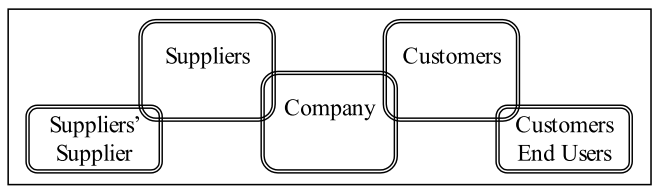
\includegraphics[width=0.80\textwidth]
		{pics/model_scm.png}
	\caption{Model \SCM}
	\label{fig:modelSCM}
\end{figure}

Dalam ilustrasi ini, \f{suppliers' suppliers} telah dimasukkan untuk menunjukkan hubungan yang lengkap dari sejumlah perusahaan atau organisasi yang bersama-sama mengumpulkan/mencari, merubah dan mendistribusikan barang dan jasa kepada pelanggan terakhir. Salah satu faktor kunci (key factor) untuk mengoptimalisasikan supply chain ialah dengan menciptakan alur informasi yang bergerak secara mudah dan akurat diantara jaringan atau mata rantai tersebut dan pergerakan barang yang efektif dan efisien yang menghasilkan kepuasan maksimal pada para pelanggan. 

%-----------------------------------------------------------------------------%
\section{Metode \f{Lot Sizing}}
%-----------------------------------------------------------------------------%
Dalam proses pengendalian persediaan barang terdapat beberapa metode \f{lotting} yang dapat digunakan. Proses \f{lotting} adalah suatu proses untuk menentukan besarnya pesanan individu yang optimal berdasarkan pada hasil perhitungan kebutuhan bersih \cite{Ibrahim}. Banyak alternatif dalam menentukan ukuran \f{lot}. Beberapa teknik untuk menambahkan ongkos pengiriman dan ongkos simpan, atau juga dengan konsep jumlah pemesanan tetap atau dengan periode pemesanan tetap. Dengan menentukan model \f{lot sizing} yang tidak tepat mengakibatkan jumlah persediaan tidak sesuai dengna kebutuhan yang sebenarnya, kelebihan persediaan juga berdampak pada meningkatnya biaya yang di timbulkan akibat barang yang masih belum terjual (tersimpan) dan mengurangi profitibilitas sebagai hasil dari penambahan modal kerja, asuransi, pajak dan keusangan. Kekurangan persediaan mengakibatkan tidak dapat memenuhi kebutuhan konsumen dan ketidak puasan konsumen akan terjadi dan mengakibatkan kehilangan kesempatan memperoleh keuntungan yang seharusnya di dapatkan.

Berikut ini beberapa metode \f{lot sizing} di antaraya sebagai berikut \cite{Almahdy}:
\begin{enumerate}
	\item \bo{\f{Lot For Lot (LFL)}}\\
	Teknik ini merupakan teknik lot sizing yang paling sederhana dan mudah dimengerti. Pemesanan dilakukan dengan pertimbangan minimasi ongkos simpan. Pada teknik ini, pemenuhan kebutuhan bersih (Rt) dilaksanakan di setiap periode yang membutuhkannya, sedangkan besar ukuran kuantitas pemesanannya (lot size) adalah sama dengan jumlah kebutuhan bersih yang harus dipenuhi pada periode yang bersangkutan. Teknik ini biasanya digunakan untuk item-item yang mahal atau yang tingkat kontinuitas permintaannya tinggi.
	
	\item \bo{\f{Fixed Order Quantity (FOQ)}}\\
	FOQ adalah sistem persedian probalistik yang variabel keputusan menggunakan Q (menotasikan kuantitas) pesanan tetap yang optimal. Kriteria optimal adalah total biaya persediaan yang minimal (Baroto, 2002). Tujuan persediaan dengan metode ini adalah untuk menentukan jumlah pesanan yang paling optimal dengan biaya yang minimal dan titik pemesanan kembali (reorder point). Prinsip FOQ atau pengendalian persediaan sistem Q adalah pemesanan dilakukan pada saat mencapai batas titik pemesanan (reorder point). Jumlah masing-masing unit produk yang dipesan sudah tetap. Namun pemesanannya dapat berbeda waktunya (kapan reorder point dapat tercapai). Jumlah persediaan yang menjadi kebutuhan selama waktu ancang-ancang dengan memperhitungkan kebutuhan yang berfluktuasi selama waktu ancang-ancang tersebut. Persediaan untuk meredam fluktuasi ini dinamakan persediaan pengaman (Tersine, 1994). Dapat dikatakan Safety stock dalam FOQ system, diperlukan untuk mengatasi adanya fluktuasi demand selama lead time. Safety stock untuk demand probabilistik dengan stockout case lost sales dimana demand yang tidak dapat dipenuhi akan dianggap hilang.
	
	\item \bo{\f{Economic Order Quantity ( EOQ )}}\\
	Russel dan Taylor (2003) menyatakan bahwa model EOQ digunakan untuk menentukan kuantitas pesanan persediaan yang meminimumkan biaya langsung penyimpanan persediaan dan biaya pemesanan persediaan. Menurut Rangkuti (2002), Model EOQ dapat diterapkan apabila asumsi-asumsi berikut ini dipenuhi:
	
	\begin{enumerate}
		\item Permintaan akan produk adalah konstan, seragam dan diketahui
		\item Harga per unit produk adalah konstan
		\item Biaya penyimpanan per unit per tahun konstan
		\item Biaya pemesanan per pesanan konstan
		\item Waktu antara pesanan dilakukan dan barang-barang diterima konstan
		\item Tidak terjadi kekurangan bahan atau back orders Rumus EOQ yang bisa digunakan adalah \equ~\ref{eq:eoqRumus} berikut:
		
		\noindent \begin{align}\label{eq:eoqRumus}
			EOQ &= \sqrt{\frac{2DS}{H}}
		\end{align}\\
		Dimana:\\
		D = Kebutuhan bahan selama satu periode\\
		S = Biaya persiapan/pemesanan setiap kali pesan\\
		H = Biaya penyimpanan per unit\\
		Setelah diperoleh nilai kuantitas pesanan optimal dengan teknik EOQ, maka model MRP dapat dilakukan dengan melakukan pesanan sebesar kelipatan dari EOQ yang lebih besar dan terdekat dengan kebutuhan bersih.
		
	\end{enumerate}

	\item \bo{\f{Period Order Quantity ( POQ )}}\\
	Teknik POQ disebut juga dengan Economic Time CycIe. Teknik POQ ini digunakan untuk menentukan interval waktu order (Economic Order Interval). Keuntungan menggunakan teknik POQ adalah dapat menghasilkan lot size order yang berbeda dalam memenuhi net requirement. Teknik POQ ini akan lebih baik kemampuannya jika digunakan pada saat biaya setup tiap tahun sama tetapi biaya carryingnya lebih rendah, (Imam, 2005).
\end{enumerate}

Pada penelitian ini metode \f{lot sizing} yang akan digunakan adalah metode \f{EOQ} berdasarkan asumsi-asumsi kajian yang telah di temukan dari penelitian sebelumnya. Metode \f{EOQ} dapat digunakan apabila pola permintaan kebutuhan bersifat terus menerus dan tingkat kebutuhan yang konstan \cite{Ibrahim, Fuad}. Metode tersebut sesuai dengan proses bisnis yang sedang berjalan.

%-----------------------------------------------------------------------------%
\section{\f{ROP (Reorder Point)}}
%-----------------------------------------------------------------------------%
Reorder point adalah sebuah titik dimana suatu pesanan baru harus dilakukan (atau persiapan dimulai). Hal ini juga di pengaruhi oleh lead time, yaitu waktu yang dibutuhkan untuk menerima kuantitas pesanan setelah pesanan dilakukan atau persiapan dimulai.

Berikut ini cara untuk mendapatkan nilai reorder point pada \equ~\ref{eq:ropRumus} \cite{Ibrahim}:
\noindent \begin{align}\label{eq:ropRumus}
	ROP &= Q \times Lt
\end{align}\\
Keterangan:\\
Q = Jumlah tingkat kebutuhan\\
Lt = Lead time

%-----------------------------------------------------------------------------%
\section{\f{Safety Stock}}
%-----------------------------------------------------------------------------%
Persediaan Pengaman (Safety stock) muncul ketika apotek dihadapkan dengan ketidakpastian akan permintaan obat sehingga akan ada kemungkinan kehabisan stok.

Untuk itu perhitungan safety stock adalah sebagai berikut \equ~\ref{eq:safeStockRumus} \cite{Ibrahim}:
\noindent \begin{align}\label{eq:safeStockRumus}
	ROPs &= ROP + (Qmax - Qr) \times Lt
\end{align}\\
Keterangan:\\
- ROPs = reorder point dengan stok pengaman\\
- ROP = reorder point semula (sebelum ada safety stock)\\
- Qmax = jumlah (tingkat) permintaan maksimal\\
- Qr = jumlah permintaan rata-rata\\
- Lt = lead time

Atau bisa juga menggunakan rumus dibawah ini \equ~\ref{eq:ssStockRumus} \cite{Ibrahim}:
\noindent \begin{align}\label{eq:ssStockRumus}
	Safety Stock (SS) = (Z) (Q) (standar deviasi leadtime)
\end{align}
Keterangan:\\
- Z = service level yang diketahui\\
- Q = jumlah tingkat kebutuhan barang\\
%-----------------------------------------------------------------------------%
\chapter{\babTiga}
%-----------------------------------------------------------------------------%
%\todo{tambahkan kata-kata pengantar bab 1 disini}


%-----------------------------------------------------------------------------%
\section{Metodelogi Peneltian}
%-----------------------------------------------------------------------------%

Pada penelitian kali ini dilakukan langkah-langkah secara terencana dan sistematis, hal ini berguna agar dapat mempermudah proses dalam pengerjaan penelitian. Metode yang digunakan dalam penelitian ini menggunakan metode tindakan karena dari tujuan peneltian ini agar memperoleh model \scm yang paling efektif dan efisien dalam mengelola bisnis dalam perusahaan atau organisasi. Adapun tahapan penelitian adalah terlihat \pic~\ref{fig:alurPenelitian} pada sebagai berikut :
\begin{figure}
	\centering
	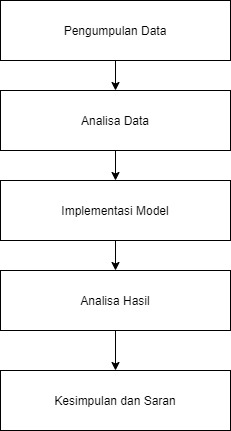
\includegraphics[width=0.40\textwidth]
		{pics/alur-penelitian.jpg}
	\caption{Metodelogi Penelitian}
	\label{fig:alurPenelitian}
\end{figure}


%-----------------------------------------------------------------------------%
\section{Pengumpulan Data}
%-----------------------------------------------------------------------------%
Pada Pada tahap pengumpulan data, penelitian ini menggunakan data primer pada sistem informasi penjualan Toko Chaca Komputer. Data yang digunakan pada penelitian ini adalah berupa data transaksi penjualan, data produk, data kategori produk dan data pelanggan. Data-data tersebut digunakan sebagai variabel-variabel yang signifikan maupun variabel pembantu yang saling berpengaruh untuk pemodelan sistem yang akan disimulasikan. Data yang terkumpul untuk selanjutnya dianalisis dan akan digunakan sebagai bahan dalam tahapan selanjutnya yaitu analisa data.

%-----------------------------------------------------------------------------%
\section{Analisa Data}
%-----------------------------------------------------------------------------%

Pada tahap analisa data, penelitian ini menggunakan data yang telah di kumpulkan untuk di analisa ulang yang akan disesuaikan dengan kebutuhan untuk kepada tahap selanjutnya.

%-----------------------------------------------------------------------------%
\section{Implementasi Model}
%-----------------------------------------------------------------------------%
Implementasi model merupakan implementasi dari data yang telah di analisa kemudian di implementasi ke model yang telah di kembangkan yang bertujuan untuk menguji model yang digunakan.

%-----------------------------------------------------------------------------%
\section{Analisa Hasil}
%-----------------------------------------------------------------------------%
Setelah melakukan implementasi model, maka tahapan yang selanjutnya dilakukan adalah melakukan analisa terhadap hasil simulasi dari pengembangan awal model sistem yang telah dibuat, kemudian dilakukan perbaikan terhadap model awal berdasarkan hasil skenario yang telah diuji coba.

%-----------------------------------------------------------------------------%
\section{Kesimpulan dan Saran}
%-----------------------------------------------------------------------------%

Tahap penyusunan kesimpulan dilakukan dengan menelaah secara keseluruhan terhadap apa yang telah dilakukan pada penelitian ini. Kesimpulan dibuat berdasarkan hasil studi literatur, desain metode penelitian, validasi data, analisis hasil simulasi dan penyusunan hasil yang diperoleh dari pengembangan model dan sistem rantai pasok barang berdasarkan produk pada toko chaca komputer. Tahap terakhir dalam penelitian ini juga menganalisis dan membahas temuan keseluruhan dalam penelitian, terkait dengan kesimpulan hasil pengujian model sistem dinamik dan saran untuk peluang penelitian yang akan datang. 
\include{bab4}
\include{bab5}
%\include{bab6}
%\include{kesimpulan}

%
% Daftar Pustaka
%
% Daftar Pustaka 
% 

% 
% Tambahkan pustaka yang digunakan setelah perintah berikut. 
% 
\phantomsection %hack to add clickable section for pustaka
%\begin{thebibliography}{4}

%\bibitem{latex.intro}
%{Jeff Clark. (n.d). \f{Introduction to LaTeX}.
%26 Januari 2010. \url{http://frodo.elon.edu/tutorial/tutorial/node3.html}.}

%\end{thebibliography}

\bibliographystyle{IEEEtran}
\bibliography{library}



%
% Lampiran 
%
\begin{appendix}
	\include{markLampiran}
	\setcounter{page}{2}
	\include{lampiran}
\end{appendix}

\end{document}